\section{Ablauf des Testprogramms}

Um den Ablauf des Testprogramms nach dem Start eines neuen Tests zu veranschaulichen, werden im Folgenden zwei Flussdiagramme präsentiert. Diese Diagramme skizzieren den 
grundlegenden Ablauf, ohne dabei auf spezifische Details des Quellcodes einzugehen.

\begin{figure}[H]
    \centering
      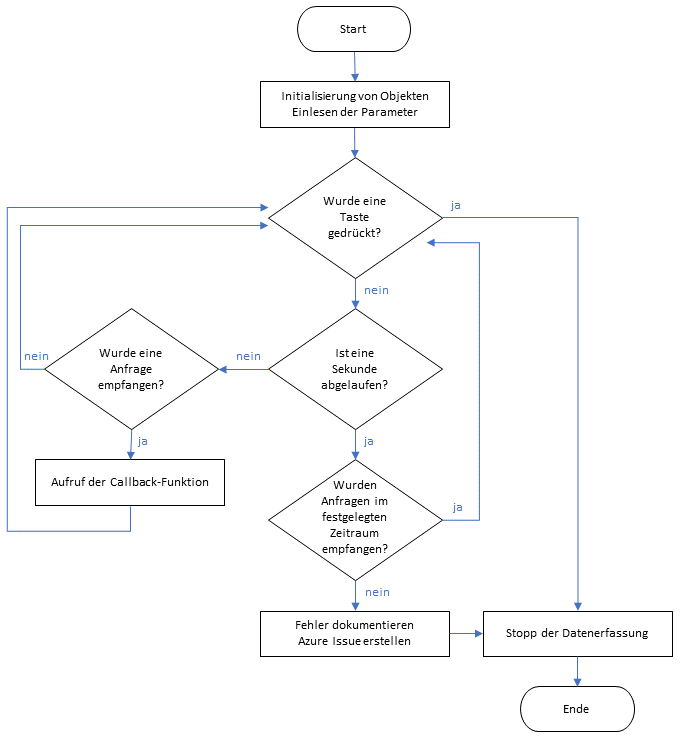
\includegraphics [width=0.68\textwidth]{mainAblauf.png}
    \caption[Flussdiagramm Hauptprogramm]{Flussdiagramm Hauptprogramm (eigene Darstellung)}
    \label{fig:mainAblauf}
\end{figure}

Das Flussdiagramm in Abbildung \ref{fig:mainAblauf} zeigt die Funktionsweise der Hauptfunktion, die zu Beginn des Testprogramms ausgeführt wird. Diese initialisiert am Anfang die benötigten Objekte, die für 
den Zugriff auf die Hilfsfunktionen notwendig sind. Anschließend wird der Logger für die Log-Datei zur Überwachung des Testprogramms erstellt, um den  Prozess nachvollziehen
zu können. Mithilfe der Klasse \glqq ConfigurationHandler\grqq\ wird die Konfiguration eingelesen sowie der Ausgabeordner erstellt (siehe Kapitel \ref{Konfigurationsdatei}). Nach 
erfolgreichem Abschluss dieser Schritte wird der Logger für die Datenübertragung und Speicherung konfiguriert, einschließlich der Festlegung des Log-Levels und der Implementierung 
der Log-Rotation. Diese Schritte setzen das vorherige Einlesen der erforderlichen Parameter voraus, da diese für die Initialisierung erforderlich sind. Im weiteren Verlauf wird das 
Gerät (RadarImager) mittels des Impact Acquire \acs{SDK} initialisiert und für die Kommunikation vorbereitet. Mit diesen Vorbereitungen ist das System bereit, mit der Datenerfassung 
zu beginnen.

Während der Datenerfassung überprüft das Programm kontinuierlich die Kommunikation. Diese Überprüfung erfolgt in einsekündigen Intervallen und stellt sicher, dass innerhalb einer 
festgelegten Zeitspanne Anfragen empfangen werden. Sollte keine Kommunikation feststellbar sein, wird das Programm abgebrochen, eine entsprechende Log-Nachricht erstellt und ein 
\glqq Azure Issue\grqq\ generiert. Solange die Kommunikation ordnungsgemäß funktioniert, bleibt das Programm in Bereitschaft, um Daten zu empfangen und die 
zugehörige Callback-Funktion auszulösen. Dies gewährleistet eine effiziente und kontinuierliche Datenverarbeitung während des Testlaufs.

\begin{figure}[H]
    \centering
      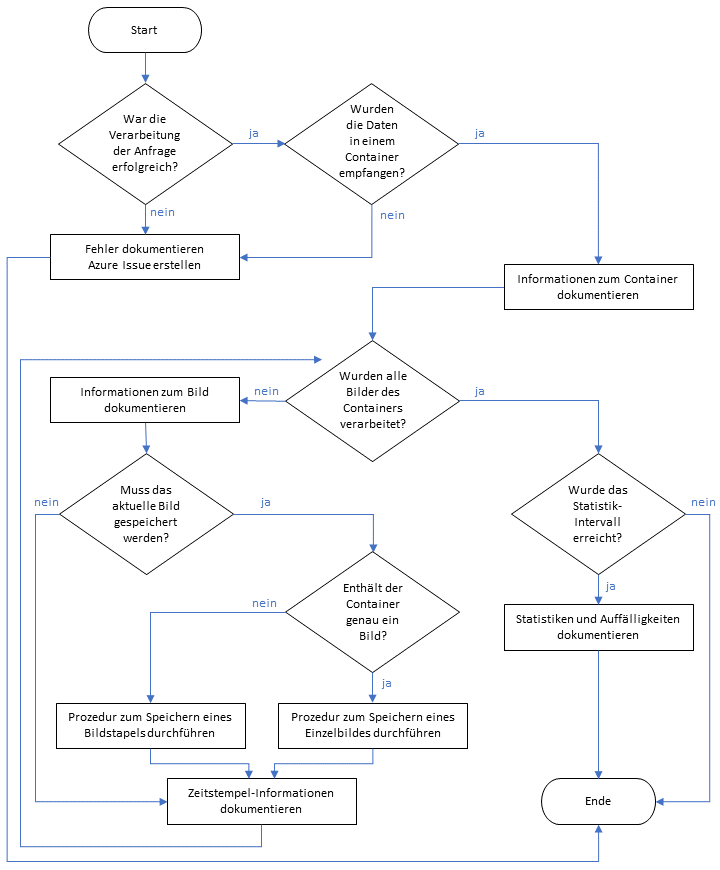
\includegraphics [width=0.7\textwidth]{requestAblauf.png}
    \caption[Flussdiagramm Callback-Funktion]{Flussdiagramm Callback-Funktion (eigene Darstellung)}
    \label{fig:requestAblauf}
\end{figure}

Die Callback-Funktion gliedert sich in zwei Hauptbereiche: Fehlererkennung und Bilddatenverarbeitung (siehe Abbildung \ref{fig:requestAblauf}). Im Bereich der Fehlererkennung werden verschiedene Eigenschaften der empfangenen 
Anfrage auf Kompatibilität mit den erwarteten Werten überprüft. Dies umfasst die Bestätigung, dass die Anfrage erfolgreich verarbeitet ist und die Daten innerhalb eines Containers 
empfangen werden. Ein erkannter Fehler führt zur Protokollierung in einer Log-Nachricht, zur Erstellung eines \glqq Azure Issues\grqq\ und zum Abbruch des Testprogramms.

Im zweiten Bereich, der Bilddatenverarbeitung, werden zunächst Informationen über den empfangenen Container im Terminal dargestellt und in den Log-Dateien vermerkt. Die Verarbeitung 
der Bilder erfolgt durch eine for-Schleife, die durch die Bilder des Containers iteriert. Für jedes Bild werden zusätzliche Informationen ausgegeben und gespeichert. 
Entsprechend den Anforderungen wird gegebenenfalls ein Speichervorgang für das aktuelle Bild initiiert. Unabhängig davon werden der Zeitstempel und die Verarbeitungszeit jedes Bildes 
in den Log-Dateien dokumentiert. Nach der Verarbeitung aller Bilder des Containers werden relevante Statistiken ausgegeben, sobald ein bestimmtes Intervall erreicht ist (siehe Kapitel 
\ref{Logging} und Abbildung \ref{fig:Logfile}). Damit ist die Callback-Funktion abgeschlossen.